\documentclass[11.5pt]{sig-alternate} % sets document style to sig-alternate
% packages
% typesetting
%\usepackage{dirtytalk} % typset quotations easier (\say{stuff})
\usepackage{hanging} % hanging paragraphs
\usepackage[defaultlines=3,all]{nowidow} % avoid widows
\usepackage[pdfpagelabels=false]{hyperref} % produce hypertext links, includes backref and nameref
\usepackage{xurl} % defines url linebreaks, loads url package
\usepackage{microtype}
\usepackage{textgreek}
%\usepackage{textcomp}
%\newcommand{\texttildemid}{\raisebox{0.4ex}{\texttildelow}}
% layout
\usepackage{enumitem} % control layout of itemize, enumerate, description
\usepackage{fancyhdr} % control page headers and footers
\usepackage{float} % improved interface for floating objects
%\usepackage{multicol} % intermix single and multiple column pages
% language
\usepackage[utf8]{inputenc} % accept different input encodings
\usepackage[english]{babel} % multilanguage support
% misc
\usepackage{graphicx} % builds upon graphics package, \includegraphics
%\usepackage{lastpage} % reference number of pages
%\usepackage{comment} % exclude portions of text (?)
\usepackage{xcolor} % color extensions
\usepackage[backend=biber, style=apa]{biblatex} % sophisticated bibliographies % necessary for HTML to display author info and date on abstract page
\usepackage{csquotes} % advanced quotations, makes biblatex happy
\usepackage{authblk} % support for footnote style author/affiliation
% tables and figures
\usepackage{tabularray}
%\usepackage{array} % extend array and tabular environments
\usepackage{caption} % customize captions in figures and tables (rotating captions, sideways captions, etc)
%\usepackage{cuted} % allow mixing of \onecolumn and \twocolumn on same page
\usepackage{multirow} % create tabular cells spanning multiple rows
%\usepackage{subfigure} % deprecated, support for manipulation of small figures
%\usepackage{tabularx} % extension of tabular with column designator "x", creates paragraph-like column whose width automatically expands
%\usepackage{wrapfig} % allows figures or tables to have text wrapped around them
%\usepackage{booktabs} % better rules
% dummy text
%\usepackage{blindtext} % blind text dummy text
%\usepackage{kantlipsum} % Kant style dummy text
\usepackage{lipsum} %lorem ipsum dummy text
% other helpful packages may be booktabs, longtable, longtabu, microtype

\pagestyle{fancy} % sets pagestyle to fancy for fancy headers and footers

% header and footer
% modern way to set header image
\renewcommand{\headrulewidth}{0pt} % defines thickness of line under header
\renewcommand{\footrulewidth}{0pt} % defines thickness of line above header
\setlength\headheight{80.0pt} % sets height between top margin and header image, effectively moves page contents down
\addtolength{\textheight}{-80.0pt} % seems to affect the lower height. maybe only works properly if footer numbers enabled?
\fancyhf{}
\fancyhead[CE, CO]{
\includegraphics[width=\textwidth]{headerImage.png}}
% footer
%\fancyfoot[LE,LO]{Article Title Here \\ DOI: }% left footer article title and doi
%\fancyfoot[CE,CO]{{}} % center footer empty
%\fancyfoot[RE,RO]{\thepage} % right footer page numbers
%\pagenumbering{arabic} % arabic (1, 2, 3) numbering in footer

\hypersetup{colorlinks=true,urlcolor=blue} % sets link color to blue
\urlstyle{same} % sets url typeface to same as rest of text

% set caption and figure to italics, label bold, left align captions, does not transfer to HTML
\captionsetup{labelfont=bf, font={large, it}, justification=raggedright, singlelinecheck=false}
\renewcommand\theContinuedFloat{\alph{ContinuedFloat}}

%this next bit is confusing, but essentially changes the width of the abstract. Seems to have been copied from this https://tex.stackexchange.com/questions/151583/how-to-adjust-the-width-of-abstract
\let\oldabstract\abstract
\let\oldendabstract\endabstract
\makeatletter %changes @ catcode to enable modification (in parsep)
\renewenvironment{abstract} %alters the abstract environment
{\renewenvironment{quotation}%
               {\list{}{\addtolength{\leftmargin}{1em} % change this value to add or remove length to the the default ?
                        \listparindent 1.5em%
                        \itemindent    \listparindent%
                        \rightmargin   \leftmargin%
                        \parsep        \z@ \@plus\p@}%
                \item\relax}%
               {\endlist}%
\oldabstract}
{\oldendabstract}
\makeatother %changes @ catcode to disable modification

% checks
% italics 
% links
% dashes
% tildes
\begin{document}

\title{Deaf Children’s Science Content Learning in Direct Instruction versus Interpreted Instruction}

\author[1]{\large \color{blue}Kim B. Kurz}
\author[1]{\large \color{blue}Peter C. Hauser}
\author[2]{\large \color{blue}Brenda Schick}

\affil[1]{Rochester Institute of Technology}
\affil[2]{University of Colorado-Boulder}

\toappear{}
%% ABSTRACT
\maketitle
\begin{@twocolumnfalse} 
\begin{abstract}
\item 
\textit{This research study compared learning of 6-9th grade deaf students under two modes of educational delivery – interpreted vs. direct instruction using science lessons. Nineteen deaf students participated in the study in which they were taught six science lessons in American Sign Language. In one condition, the lessons were taught by a hearing teacher in English and were translated in ASL via a professional and certified interpreter. In the second condition, the lessons were taught to the students in ASL by a deaf teacher. All students saw three lessons delivered via an interpreter and three different lessons in direct ASL; the order of delivery of each presentation was counter balanced between the two groups of students. Following the instruction, each group was tested on the science lecture materials with six comprehension questions. Results indicated that deaf students who received direct instruction in ASL from the deaf teacher scored higher on content knowledge.}
\\ \\
Keywords: Science Education, Deaf Education, American Sign Language, Direct Communication, Educational Interpreter
\end{abstract}
\end{@twocolumnfalse}

%% AUTHOR INFORMATION

\textbf{*Corresponding Author, Kim B. Kurz}\\
\href{mailto:  kim.kurz@rit.edu}{(kim.kurz@rit.edu)} \\
\textit{Submitted Jul 16 2015 }\\
\textit{Accepted Aug 24 2015} \\
\textit{Published online  Oct 9 2015} \\
\textit{DOI:10.14448/jsesd.07.0003} \\
\pagebreak
\clearpage
\begin{large}
\section*{INTRODUCTION}
    
Picture a classroom in a school district where a teacher is explaining the skeletal system of a prehistoric dinosaur. The teacher has a model of the Tyrannosaurus Rex on a table and is pointing out each bone in the dinosaur. The Smartboard has a projected list of the names of various bones and their relative sizes. Each student has a worksheet in front of them and they are labeling the bones. Twenty-six fifth graders have their eyes glued to the teacher, the model, and the Smartboard. The twenty-seventh student is looking back and forth between the model, the screen, the worksheet, and another adult. The other adult who draws her focus is her educational interpreter. The twenty-seventh student is deaf, and she watches the interpreter who is translating the teacher’s spoken lecture into American Sign Language.

This study examines the deaf and hard of hearing middle school students’ learning experience in science education between educational situations where the information is communicated directly and through a certified sign language interpreter. The primary research question was, “Do deaf students learn different amounts of information in direct communication conditions compared to interpreted conditions using science lessons?”. The secondary research question was whether the deaf students’ language background made a difference in their comprehension of the science lessons in one or both conditions.

\subsection*{Science Education for Deaf and Hard of Hearing Students}

Lane-Outlaw (2009) describes, “In ASL/English bilingual secondary science classrooms, teachers use both languages to teach concepts and skills to students, but little is known about how this instruction is accomplished” (p. vii).  We know very little about effective teaching approaches and how deaf children learn both languages, English and ASL, in bilingual classrooms. Erting (2001) explains that deaf students arrive at school without the same background knowledge and linguistic skills as their hearing peers. This often leads to an educational focus on language instruction. Lane-Outlaw (2009) explains that too often deaf education programs focus on teaching language other than science which is also an important life skill in understanding how science works around us in this world. Without integrating content knowledge and language instruction, deaf students fall further behind in content knowledge (McIntosh, Sulzen, Reeder, \& Kidd, 1994).  Sunal and Burch (1982) suggest that the deaf education programs build science knowledge on top of teaching language, cognitive and developmental skills. 

There is not much research on science education with deaf students (Mangrubang, 2004; Moores, Jathro, \& Creech, 2001). The research that has been conducted related to science education with deaf students in general has not looked specifically at science instruction or language use, yet many of the recommendations for future research include investigating the use of sign language in science instruction (Molander, Pedersen \& Norell, 2001; Roald, 2002; Roald \& Mikalsen, 2000; Sunal \& Burch, 1982). While there have been numerous studies conducted related to reading and language instruction with deaf students, very little research has been conducted on deaf students' language, literacy, or instruction in content areas (Lane-Outlaw, 2009). 

\subsection*{Today’s Deaf and Hard of Hearing Students}

Today, a majority of deaf and hard of hearing children in America receive    educational services under the current federal laws. The most recent Gallaudet Research Institute Annual Survey of deaf and hard of hearing children and youth’s national data in 2011-2012 shows that 23,700 deaf and hard of hearing students were identified in the country. Approximately 68\% of these students were currently attending mainstreamed programs, 22\% were attending schools for the deaf (Gallaudet Research Institute, 2012). Of the deaf and hard of hearing students who are mainstreamed, 58\% of students were fully mainstreamed with their hearing classmates, 2-6\% were enrolled in self-contained classrooms and the remaining 16\% of mainstreamed students used resource classrooms to aid them with their studies (Gallaudet Research Institute). A form of educational service is the use of educational interpreters who work in K-12 school settings. At least 14\% of mainstreamed deaf and hard of hearing students had sign language interpreters in their classrooms (Gallaudet Research Institute). 

\subsection*{Educational Interpreting and Science Education}

Research interest in learning through sign language interpreting has emerged in the more recent years (see Kluwin \& Stewart, 2000; Mar\-schark, Sapere, Convertino, \& Seewagen, 2005; Stewart \& Kluwin, 1996). In general, some people are led to believe that interpreted instruction is equal, in amount of information delivery, compared to direct instruction (i.e., the teacher provides information directly to the student in the students’ primary language). There is a huge assumption that language access through an interpreter is complete and that interpreters are adequate language models for deaf children, but many professionals who are knowledgeable about interpreting dispute this (Hopper, 2011; Ramsey 1997; Schick, Williams \& Bolster, 1999). The assumption is that providing educational interpreters for deaf and hard of hearing students in mainstreamed settings is adequate. However, Schick (2004) argues, “educating children with the use of an interpreter is (still) an educational experiment” (p. 73). 

Literature regarding educational interpreting provides considerable information about the qualifications and roles of interpreters and the various interpreter preparation programs. Information regarding how deaf and hard of hearing students benefit from being in an interpreted educational setting within science education is limited (Jones, Clark, \& Soltz, 1997). In Solomon’s (2012) whitepaper based on input from those who attended the National Science Foundation’s two-day event, “Workshop for Emerging Deaf and Hard of Hearing Scientists” May 17-18, 2012, it states that many of the challenges faced by deaf students and professionals are related to the lack of qualified and experienced interpreters which has an effect on their access to communication.   Graham, Solomon, Marchut, Kushalnagar, \& Painter (2012) describes that deaf and hard of hearing students reported difficulty in following lecturers with those interpreters who did not have scientific training. We need to be able “to identify the skill set, knowledge base, and other attributes that sign language interpreters must possess in order to provide effective services for deaf professionals in the STEM fields” (Grooms, 2015). 

Napier \& Barker (2004) found that deaf students do not comprehend as much as we or they think they do from interpreted lectures. Grooms (2015) states that “there has been no research to date regarding STEM interpreting as a specialty in the field” and recommends that Interpreter Preparation Programs consider adding STEM as a specialty in addition to the other six most common areas of specialization. Those six areas of specialization for interpreters were identified as 1) legal, 2) medical, 3) mental health, 4) K-12 education, 5) post-secondary education settings, and 6) providing services for people who are Deaf-Blind (Walker \& Shaw, 2012). Grooms (2015) also states “Research on interpreting in the STEM fields should focus on the experiences of Deaf students and professionals in the STEM disciplines and their experiences with interpreters to tease out the necessary competencies interpreters must have to provide effective services in those disciplines”.

Literature clearly shows that deaf and hard of hearing students need competent interpreters as some of them might choose science as their chosen career. Little research exists on how deaf students learn and process information using a third party – the interpreter—in the science classroom. 

\subsection*{The Educational Interpreter Performance Assessment (EIPA)}

The Educational Interpreter Performance Assessment (EIPA) is a metric tool designed to evaluate the voice-to-sign and sign-to-voice interpreting skills of interpreters who work in elementary and secondary school classroom settings (Schick, Williams, \& Bolster, 1999). The EIPA assesses performance skills of interpreters working in K-12 educational settings. The EIPA rates interpreters on a scale of 1-5 in 36-38 different skill areas. Educational interpreters who score in the 3.5 – 4.0 range, while often quite competent, miss some information and inaccurately convey other information. Recent analysis of EIPA data demonstrated that 63\% of EIPA evaluations (\textit{n} = 8, 680) were 3.5 or higher (3.5 is a common state minimum standard; Johnson, Schick, and Bolster, 2014; see also Schick, Williams, \& Kupermitz, 2006). Schick et al. (2006) also found that the average EIPA score (0-5 scale) for individuals who attended an interpreter training program versus those who had not, and those with and without a bachelor’s degree, did not show significant statistically different between these groups. A recent analysis of data from the Educational Interpreter Performance Assessment database (EIPA; Johnson, Schick, \& Bolster, 2014) collected and evaluated more than 18,000 EIPA evaluations from 2002 to 2014. While we have a fairly good idea of what our current educational interpreters’ skills are today, we are still learning more about how deaf children learn through educational interpreters and teachers in educational settings.

Based on the literature review, there is very little information related to what we know about how deaf and hard of hearing students learn science lesson materials through direct communication using ASL and a certified sign language interpreter. The researchers wanted to find out by conducing a study in this area. As the field of STEM (Science, Technology, Engineering and Math) continues to grow and become an even more important subject leading to jobs and career pathway for deaf and hard of hearing population in the future, the researchers wanted to learn more about how much deaf and hard of hearing students are able to acquire information related to science lesson materials through both conditions – direct communication via American Sign Language and through a sign language certified interpreter.

\section*{METHOD}

\subsection*{Participants}

The participants in this study included a total of 19 individuals who were between the ages of 11 and 15 years and between the grade levels of 6th and 9th grade (see Table 1). Twelve participants were from direct communication environments (i.e., residential schools for the deaf and day schools for the deaf) and seven participants were in mainstreamed programs with interpreters (i.e., public school). Five native-signing participants who were raised by deaf and signing parents and seven non-native signing participants who were born to hearing parents who learned sign language after they were born were from the direct communication environments, and four native signing participants and three non-native signing participants were from the mainstreamed programs. Sixteen participants reported the use American Sign Language (ASL) as their primary communication mode, two participants use contact signing, and one participant uses both ASL and contact signing.

\begin{table}[h]
\caption{Students’ demographic information}
\begin{tabular}{lcc}
\hline
& Native Signers (\textit{n} = 10) & Non-native Signers (\textit{n} = 9) \\ \hline
Mean Age (\textit{SD}) & 13.1 (1.5) & 13.4 (0.9) \\
Gender (\textit{n}) & & \\
Female & 4 & 6 \\
Male & 6 & 3 \\
Grade (\textit{n}) & & \\
6th & 1 & 1 \\
7th & 5 & 3 \\
8th & 1 & 3 \\
9th	& 3 & 2 \\ \hline
\end{tabular}
\end{table}

\subsection*{Materials}

The researchers recruited a certified general education hearing teacher who taught science at the middle school level, and a certified teacher of the deaf, secondary-level, who had undergraduate education in mathematics and science. The hearing teacher had a master’s degree in ecology and had eight years of science teaching experience at a middle school. The deaf teacher is a native user of ASL and had seven years of experience teaching math and science to both deaf and hearing students at the secondary and postsecondary levels. An interpreter who was certified by the Registry of Interpreters for the Deaf (RID) and had several years of interpreting full-time at the secondary level in an educational setting was identified. The interpreter holds a Certificate of Interpretation (CI) and Certificate of Transliteration (CT) from the RID with a 5.0 EIPA certification level (the highest possible level given by EIPA). The interpreter is a native signer, a child of deaf adults (her first language is ASL) with more than twenty-five years of interpreting experience.

First, six lesson plans were developed about science topics that were not commonly used in today’s science curriculum, but at the same time contained information that was appropriate for participants at the middle school level. The lessons were designed for participants to be able to follow the instruction relatively easily. The six science topics were as follows: (1) Conservation Tillage; (2) Importance of Trees in Rural Areas: Living Snowfences; (3) Reef-building Corals; (4) How Islands Form; (5) Forensic Archaeology; and (6) Radioactive Dating. Once the six lesson plans were developed with input from both science teachers, pre-tests and post-tests were developed.

There were six questions for each lesson with a total of thirty-six questions across the six lessons. For example, in the “How Island Form” section, the six questions that were asked during pre-test and post-test are: 1) How did New Zealand become isolated from the mainland of Australia?; 2) How did the Florida Keys appear?; 3) Imagine you are a scientist, someone asks you how islands are formed. How would you explain it to that person? Be sure to include two different ways of island formation.; 4) How do the geological and geographical features of islands affect the people who live on them?; 5) Hypothesize about the effect a future ice age would have on the world’s largest islands and their plants and animals; and, 6) How long do you think it takes to form islands? Justify your thoughts.  

A rubric for the first question, “How did New Zealand become isolated from the mainland of Australia?” include points that range from 0 to 4. An example of the rubric include some possible answers to earn points on the measurement scale include: 4 Points – “Some bodies of land were cut off from the mainland and became islands. For example, there are the polar ice caps on the map. During the last ice age the ice caps were larger. More of Earth’s water was frozen at the poles, and the oceans were shallower. Sea levels rose dramatically at the end of the Ice Age as Earth warmed and the polar ice caps began to melt. When the ice melted, about 10,000 years ago, some bodies of land that had been connected to continents were cut off from the mainland and became islands. This is how the islands of New Zealand became isolated from the mainland of Australia”; 3 Points – “Sea levels rose dramatically at the end of Ice Age as Earth warmed and the polar ice caps began to melt. When the ice melted, about 10,000 years ago, some bodies of land that had been connected to continents were cut off from the mainland and became islands”; 2 Points – “When the ice melted, about 10,000 years ago, some bodies of land that had been connected to continents were cut off from the mainland and became islands.”; 1 Point – “Sea levels rose and cut off some land from island.” or “It happened 10,000 years ago.”, and 0 Point – Blank/No response, “I don’t know” response or incorrect response such as “There was an earthquake and the plates moved”. For full information related to all questions and rubric measurements, see Kurz (2004).

Finally, the last phase was to produce videotapes of the lectures. Both the hearing teacher/inter\-preter and deaf teacher used exactly the same scripts that were written in English for all six lesson plans. The deaf teacher translated the English version script/lesson into ASL and the hearing teacher translated the English version script/lesson into spoken English. The interpreter did not have prior access to the lessons/scripts. The teachers on the video provided some lecture and then periodically throughout the lessons asked the 36 questions. The hearing teacher taught each lesson with an interpreter interpreting the lessons. The interpreter had a copy of the lesson plans prior to interpreting as is the accepted best practice procedure for educational interpreters. 

\subsection*{Procedure}

All participants were given pre- and post-tests to measure their knowledge and understanding of the subject prior to and after receiving the lesson. The participants were seated in front of the TV monitor, the procedures were explained to them (i.e., what they would be viewing and what they were to do), and that the participants would be videotaped for subsequent analysis of their answers by the researcher. The researcher would stop the video each time the teacher asked a question to avoid problems with long-term memory. It was determined that if the participant had to wait until the end of each lesson presentation to respond to the questions, they might forget the information and this could influence their post-test answers. All participants were tested individually. The test stimuli were consisted of lectures which were not interactive. The lectures were didactic in nature. 

All participants received the baseline condition in the same way. The six knowledge questions for each lesson were asked and the participants’ baseline knowledge scores on these questions provided the pre-test information. Second, the treatments  (Treatment B = Direct Communication, Treatment C = Interpreted Education) were implemented and counter-balanced with each subject receiving each treatment three times (three lessons were provided in either direct or interpreted format for a total of six lesson plans). For example, one subject received the treatments in a Baseline (Pre-Test) then B-C-B-C-B-C order while the other subject received the treatments in a Baseline (Pre-Test) then C-B-C-B-C-B sequence. Nine participants received the first lesson presentation order and ten participants received the second presentation order. The participants were randomly assigned to the order presentation. After the participants viewed the lectures, they were asked the same 36 pre-test questions during the post-test. All participants gave their answers in ASL during pre-test and post-test. Their answers were recorded by a camcorder and translated into written English to document their answers into an Excel spreadsheet.

A rubric was developed for each question in each science lesson. The rubric was used to measure the subject’s acquisition of knowledge in both pre-tests and post-tests. The rubric scale for accuracy ranged from 0 to 2. “0” meant the answer was either incorrect or “I don’t know”, “1” meant the answer was somewhat correct but not fully correct, and “2” meant the participant received full credit for correct answers. The observer and reliability observer used the rubrics to assign scores and the science teachers provided consultation for the rubrics to ensure that each answer received a fair score. The overall percentage of inter-observer agreement for student-by-lesson plan was 93.1%.

\section*{RESULTS}

A repeated measures ANOVA was used to determine if the participants learned more information in one of the two Learning Situations (Direct Communication; Interpreted Education). Test (Pre-test, Post-test) was used as the repeated measure and the Learning Situations were used as within subject factors. Analyses revealed that all participants performed better on the post-test compared to their pre-test performance, \textit{F}(1,18) = 120.551, \textit{p} < .001. The effect size (η2 = .870) indicated that the magnitude between the pre- and post–scores was large. As a group, the children learned from the lectures. There were no significant differences between the participants’ Pre-Test performance, but analyses of their Post-Test performance revealed that the participants learned more in the Direct Communication (Post-Test \textit{M} = 26.95, \textit{SD} = 9.49) than in the Interpreted Education condition (Post-Test \textit{M} = 17.05, \textit{SD} = 8.96), \textit{F}(1, 18) = 21.166, \textit{p} < .001. The effect size (η2 = .543) indicated that that the magnitude of the difference was moderate. There was a significant Test x Learning Situation interaction, \textit{F}(1, 18) = 28.166, \textit{p} < .001, where the difference between the two Learning Situations were evident in the post-test condition but not in the pre-test condition (see Figure 1). The effect size (η2 = .610) was moderately strong indicating that children learn much better in the Direct Communication condition. 

\begin{figure}[h]
    \centering
    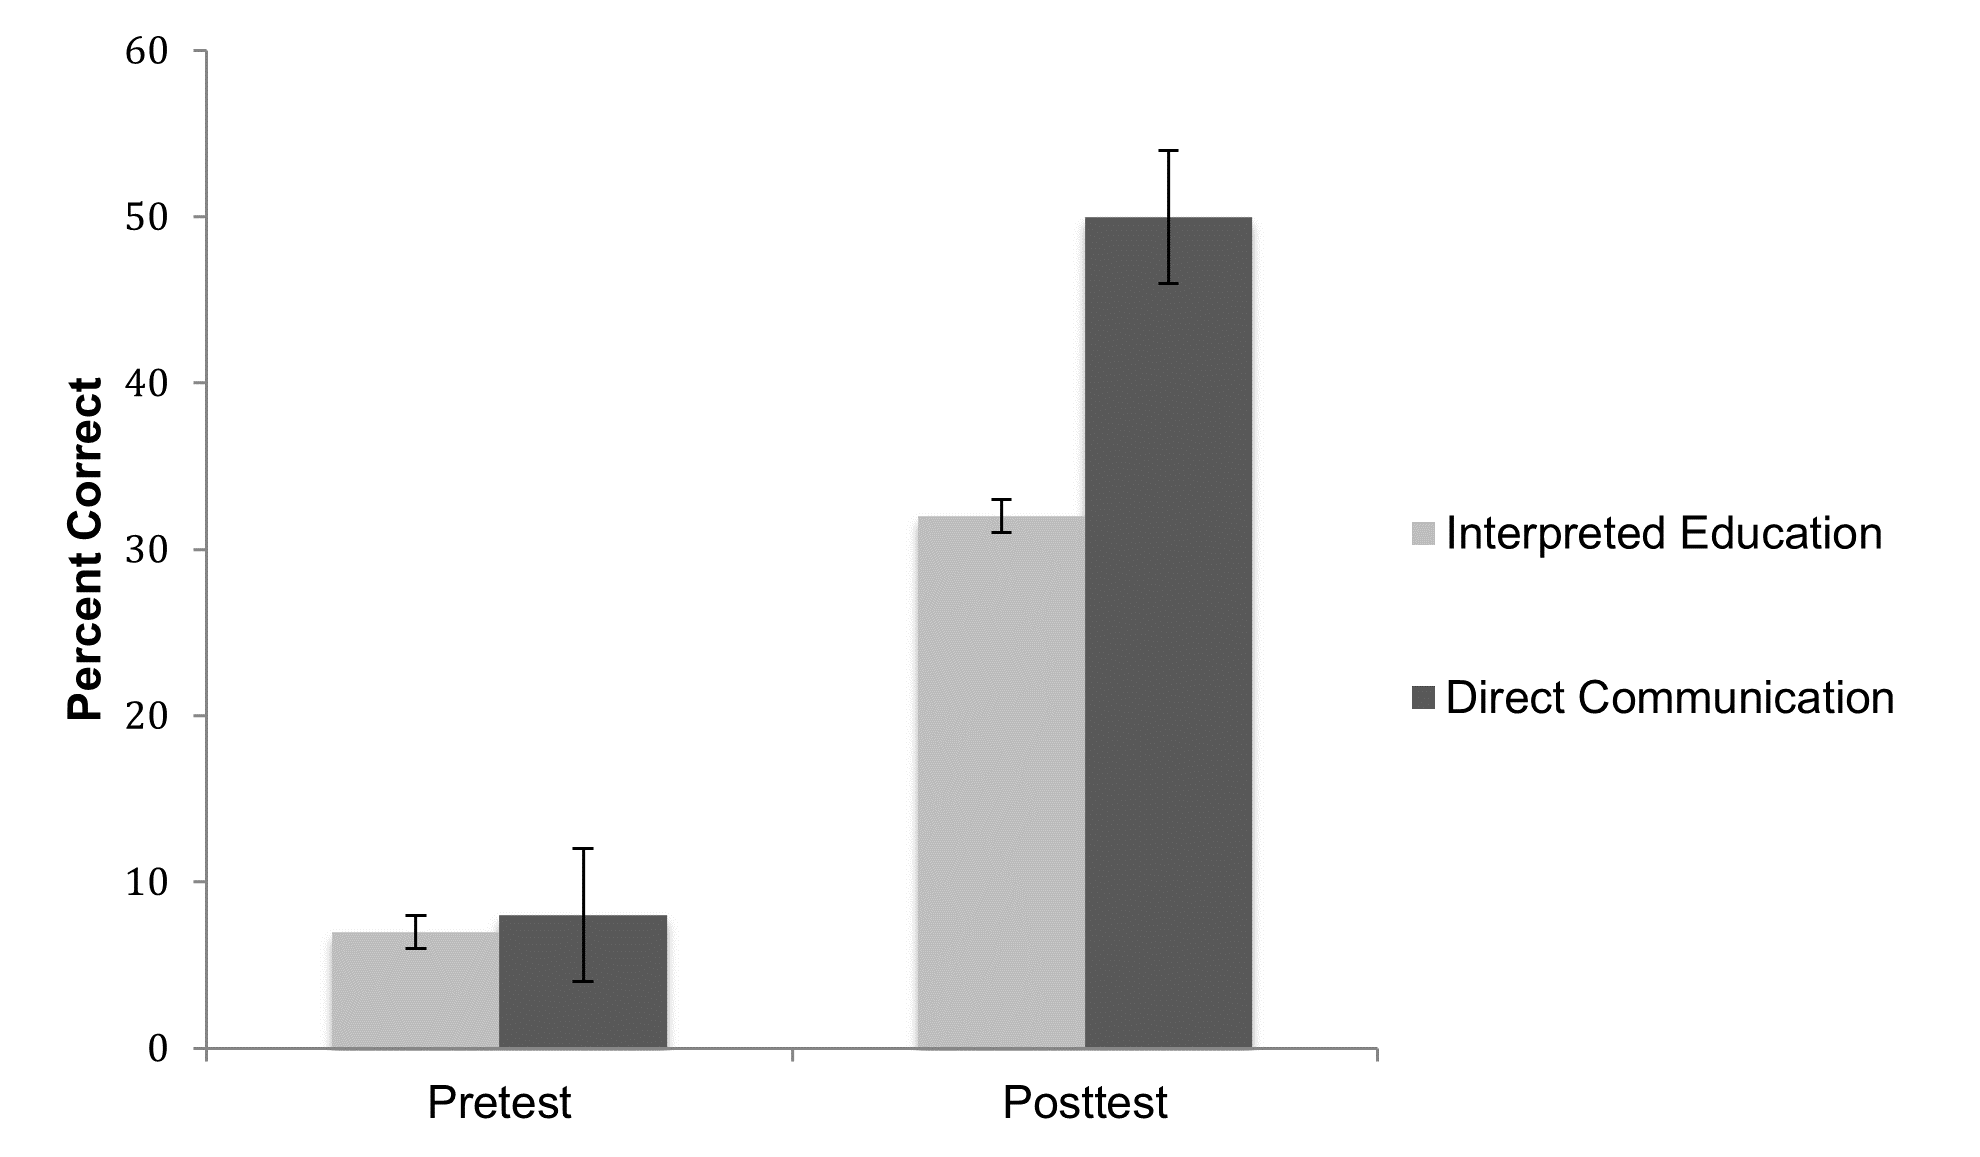
\includegraphics[width=1\linewidth]{images/fig1.png}
    \caption{Participants’ performance on the science Pre-test and Post-test in the two learning situations. Error bars represent the standard error of the mean.}
\end{figure}

To explore whether or not participants’ language background made a difference in how much they benefitted from each of the two Learning Conditions, we compared the results of the students who had deaf parents (Native Signers) and those who had hearing parents (Non-native Signers) (see Table 2 for Means and SD). A repeated measures ANOVA was used with Test (pre-test, post-test) as the repeated measure, Learning Situation (Direct Communication; Interpreted Education) as the within subject factor, and Sign Skills (Native, Non-Native) as the between subject factor. There was a significant main effect for Test where all participants performed better on the Post-test, \textit{F}(1, 17) = 144.016, \textit{p} < .001, η2 = .894. There was a significant main effect for Learning Situation where all participants performed better in the Direct Communication condition better than in the Interpreted Education condition, \textit{F}(1, 17) = 20.494, \textit{p} < .001, η2 = .547. The Native Signers performed better than the Non-native Signers in both Learning Situations, \textit{F}(1, 17) = 8.205, \textit{p} < .05. There was a small to moderate effect size (η2 = .326) indicating that although there were differences between the native and non-native signers, the difference was not large. There was no significant interaction between Sign Skills and Learning Situation or between Sign Skills, Learning Situation, and Test. However, there was a significant interaction between Test and Learning Situation where participants performed better in the Post-Test condition in the Direct Communication situation, \textit{F}(1, 17) = 26.639, \textit{p} < .001, η2 = .610 (see Figure 2). 

The differences in learning between the two Learning Situations by each participant can be seen in Figure 3, which shows a student’s performance difference for Direct minus Interpreted post test results.  Bars above zero indicate the student did better in the Direct Condition.  Bars extending below zero indicate that the student did better in the Interpreted Condition.  As can be seen, there are large individual differences among the participants, but in general, the majority of the students did better in the Direct Condition.

\begin{table*}[th]
\caption{Participants Mean raw scores on Pre-Tests and Post-Tests in the two Learning Situations}
\begin{tabular}{lcccc}
\hline
& \multicolumn{2}{c}{Interpreted Education} & \multicolumn{2}{c}{Direct Communication} \\ \hline
& Pre-Test & Post-Test & Pre-Test & Post-Test \\
Non-native Signers & 2.33 (1.80) & 12.44 (5.98) & 3.56 (1.94) & 22.33 (10.16) \\
Native Signers & 5.40 (2.63) & 21.20 (9.40) & 4.80 (3.39) & 31.10 (6.92) \\ \hline
\end{tabular}
\textit{Note: Max raw score = 36; Standard Deviations are in parentheses.} 
\end{table*}

\begin{figure}[h]
    \centering
    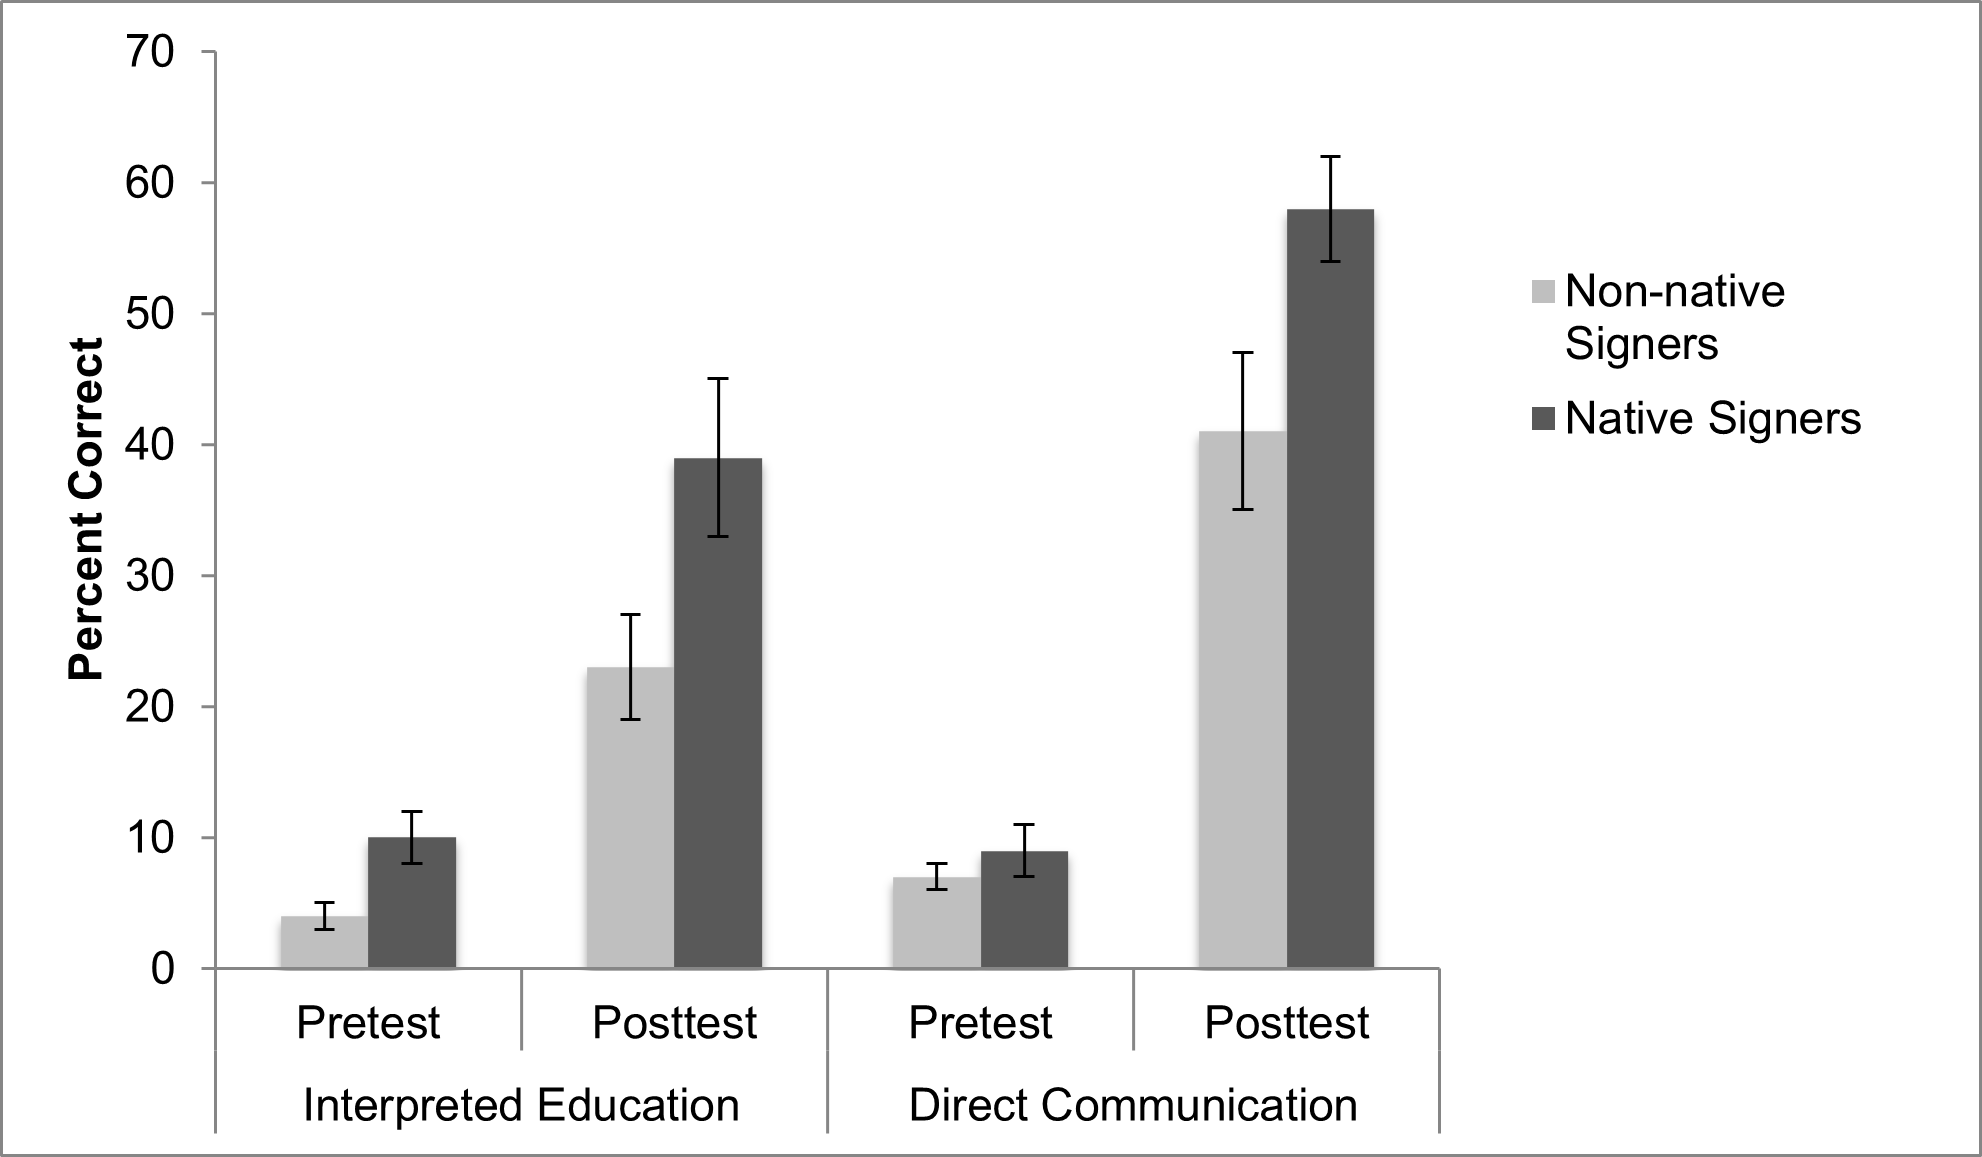
\includegraphics[width=1\linewidth]{images/fig2.png}
    \caption{Native and Non-Native signers’ performance on the science Pre-test and Post-test in the two learning conditions. Error bars represent the standard error of the mean}
\end{figure}

\begin{figure}[h]
    \centering
    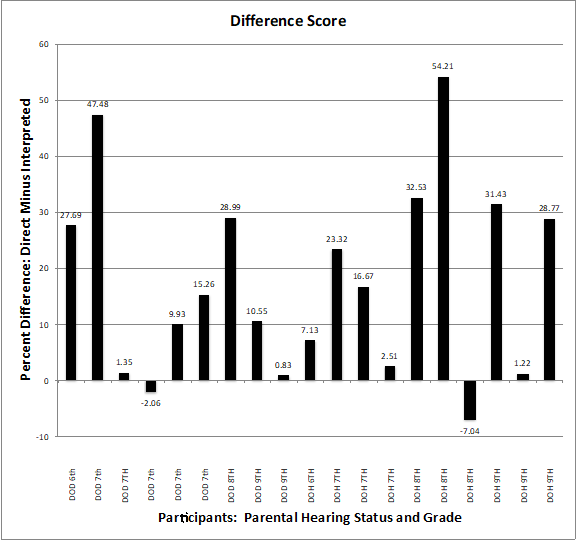
\includegraphics[width=1\linewidth]{images/fig3.png}
    \caption{Percentage difference in learning between the two Learning Situations by each participant. Note: DOD = Deaf of Deaf/Native Signer; DOH = Deaf of Hearing/Non-native signer.}
\end{figure}

These results suggest that all students can learn in both Direct Communication and Interpreted Education settings. However, even with a highly skilled interpreter, most students learned more in the Direct Communication Condition. Students who acquired sign language since birth from their deaf parents appear to be more prepared to learn in both Direct Communication and Interpreted Education conditions.

\section*{DISCUSSION}

The native signer participants, regardless of the type of school they attended, acquired, in general, more information in both interpreted and direct communication environments than did their non-native signing peers. The interpreter in this study was highly qualified; she was a native signer (CODA), had an EIPA score of 5.0, and RID CI/CT certifications, with experience working as an educational interpreter in middle schools. However, we know that the typical educational interpreter does not have these credentials and it is probable that many deaf children have access to less than optimal interpretered lectures or interpreted classroom discourse. Therefore, many deaf students are probably missing out on significant amounts of information in their classes. The interpreter not conveying complete information combined with the fact that simply learning through an interpreter appears to be more challenging, suggests that an interpreted education may not provide a deaf student access to classroom content equal to what a hearing student experiences. 

Both native signers and non-native signers did better in direct communication compared to the interpreted communication setting. It is also clear that students can vary in how well they can learn from an interpreted education.  This has major implications for school systems in that it cannot be assumed that all students will benefit from an educational placement with an interpreter.  When a deaf student is not making adequate progress in an interpreted setting, it should be determined whether the interpreted placement, rather than the student’s language and academic skills, is a barrier to learning. 

The present study has three main limitations. First, there are a relatively small number of subjects used in this study. This small sample might not be a true representation of the entire deaf student population’s education today. A larger sample of similar study is needed to better understand the implications of deaf students’ comprehension of content produced by educational interpreters. The second limitation is that the participants’ backgrounds were not entirely examined. Their written and sign language skills were not objectively measured; however, their language preferences were noted. To address this limitation in future research, it is recommended that deaf students who participate in research like this be tested for their sign language skills using current sign language skills assessment instruments.

Replication of this study is needed to better understand the implications of what and how deaf children learn through educational interpreters in their mainstreamed environments and compare it to learning in direct communication settings. Future research studies may include Certified Deaf Interpreters in order to investigate whether that would improve learning outcomes. This study also included middle school students. Replication of this study with a wider range of ages would provide information about when children are capable of learning through an educational interpreter. It is also recommended that researchers and educators need to evaluate the delivery strategies used by teachers/interpreters such as fingerspelling, content signs, use of space and depicting verbs in the area of science.

\section*{CONCLUSION}

The majority of young deaf children are being placed in mainstreamed educational settings today. This placement may represent an experiment among special education administrators, parents, and teachers of the deaf. We do not know enough about whether the mainstreamed experience with an educational interpreter provides an learning experience for a deaf child as for their hearing peers or in terms of direct access to an educator as envisioned by the Congress and lawmakers when they passed IDEA. There has been little research comparing their knowledge acquisition to that of their deaf peers in direct communication environments. This study indicates that for this group of middle school deaf students, direct communication was the better approach for acquiring new information even when the interpreter was far more qualified than what we typically see in today’s educational settings. A strong language foundation and world knowledge may be some of the most important indicators for a successful educational experience. In summary, Schick (2008, p. 351) suggests “…as an educational practice, educational interpreting is widespread, but it is not evidence-based practice.” Based on the results of the present and previous studies, we recommend further studies in this area to establish a nation-wide standard for screening students to see whether they are a good fit for direct communication or a mainstreamed setting in the future. 


\section*{ACKNOWLEDGEMENTS}
The authors would like to thank the following individuals who provided consultation and support for this research project: Dr. Sally Roberts, Rutherford Turnbull, J.D., Dr. Christopher Kurz and Dr. Ronald Kelly, and Nikki Cherry for her editorial assistance. Correspondence concerning this article should be addressed to Kim B. Kurz, Department of American Sign Language and Interpreter Education, National Technical Institute for the Deaf, Rochester Institute of Technology, Rochester, New York 14623 e-mail: \href{mailto:  kim.kurz@rit.edu}{(kim.kurz@rit.edu)}

\end{large}
\clearpage
\section*{REFERENCES}\par 

\leftskip 0.25in
\parindent -0.25in 
Erting, L. (2001). Language and literacy development in a preschool for deaf children: A qualitative study. Doctoral dissertation, University of Maryland.

Gallaudet Research Institute. (2012). National Data [data file]. Retrieved November 9, 2014 from \url{https://research.gallaudet.edu/Demographics/}

Graham, S., Solomon, C., Marchut, A., Kushalnagar, R., \& Painter, R. (2012). Experiences of students in STEM. In Solomon, C. (Ed.). Workshop for emergining deaf and hard of hearing scientists [whitepaper] (pp. 13-19). Washington, D.C.: Gallaudet University.

Grooms, C. (2015). Interpreter Competencies in Science, Technology, Engineering, and Mathematics as Identified by Deaf Professionals. Master’s Thesis, Western Oregn University.

Hopper, M. (2011). \textit{Positioned as bystanders: Deaf students’ experiences and perceptions of informal learning phenomena} (Unpublished doctoral dissertation). University of Rochester, Rochester, NY.

Johnson, L., Schick, B., \& Bolster, L. (October, 2014). EIPA Data Analysis: K-12 Patterns of Practice. Poster session presented at the meeting of the Conference of Interpreter Trainers, Portland, OR.

Jones, B.E., Clark, G.M., \& Soltz, D.E. (1997). Characteristics and practices of sign language interpreters in inclusive education programs. \textit{Exceptional Children, 63}, 257-268.

Kluwin, T. N., \& Stewart, D. A. (2000). Interpreting in schools: A look at research. \textit{Odyssey (Gallaudet University, Washington, DC)}, 15-17.

Lane-Outlaw, S. L. (2009). \textit{A qualitative investigation of ASL/English bilingual instruction of deaf students in secondary science classrooms}. GALLAUDET UNIVERSITY.

Mangrubang, F. R. (2004). Preparing elementary education majors to teach science using an inquiry-based approach: The Full Option Science System. \textit{American annals of the deaf, 149}(3), 290-303.

Marschark, M., Sapere, P., Convertino, C., \& Seewagen, R. (2005). Access to postsecondary education through sign language interpreting. \textit{Journal of Deaf Studies and Deaf Education, 10}(1), 38-50.

McIntosh, R. A., Sulzen, L., Reeder, K., \& Kidd, D. H. (1994). Making science accessible to deaf students: The need for science literacy and conceptual teaching. \textit{American annals of the deaf, 139}(5), 480-484.

Moores, D., Jathro, J., \& Creech, B. (2001). Issues and trends in instruction and deafness. American Annals of the Deaf 1996 to 2000. American Annals of the Deaf 146(2), 72-76.

Molander, B. O., Pedersen, S., \& Norell, K. (2001). Deaf pupils' reasoning about scientific phenomena: School science as a framework for understanding or as fragments of factual knowledge. \textit{Journal of deaf studies and deaf education, 6}(3), 200-211.

Napier, J., \& Barker, R. (2004). Accessing university education: Perceptions, preferences,and expectations for interpreting by deaf students. \textit{Journal of Deaf Studies and Deaf Education, 9}(2), 228-238.

Ramsey, C. (1997). \textit{Deaf children in public schools}. Washington, DC: Gallaudet University Press.

Roald, I., \& Mikalsen, O. (2000). What are the Earth and the heavenly bodies like? study of objectual conceptions among Norwegian deaf and hearing pupils. \textit{International Journal of Science Education, 22}(4), 337-355.

Roald, I. (2002). Norwegian deaf teachers’ reflections on their science education: Implications for instruction. \textit{Journal of Deaf Studies and Deaf Education, 7}(1), 57-73.

Schick, B. (2004). How might learning through an interpreter influence cognitive 	development? In E.A. Winston (Ed.), \textit{Educational interpreting: How it can succeed} (pp. 73-87). Washington, DC: Gallaudet University Press.

Schick, B. (2008). A model of learning in an interpreted education. In M. Marschark \& P. Hauser (eds.), \textit{Deaf cognition:  Foundations and outcomes} (pp. 351-386). Oxford University Press.

Schick, B., Williams, K., \& Bolster, L. (1999). Skill levels of educational interpreters working in public schools. \textit{Journal of Deaf Studies and Deaf Education, 4}(2), 144-155.

Schick, B., Williams, K., \& Kupermintz, H. (2006). Look who’s being left behind: Educational Interpreters and access to education for deaf and hard of hearing students. \textit{Journal of Deaf Studies and Deaf Education, 11}, 3-20.

Solomon, C. Ed. (2012). Workshop for emerging deaf and hard of hearing scientists [Whitepaper]. Washington, D.C.: Gallaudet University. Supported by the National Science Foundation under CNS-0837508 and MCB-1232380. Accessed at: \url{http://doit-prod.s.uw.edu/accesscomputing/sites/default/files/manual-upload/WhitePaper-Final_Gallaudet_Emerging_Sei_2_15_13.pdf}

Stewart, D. A., \& Kluwin, T. N. (1996). The gap between guidelines, practice, and knowledge in interpreting services for deaf students. \textit{Journal of Deaf Studies and Deaf Education, 1}(1), 29-39.

Sunal, D. W., \& Burch, D. E. (1982). School science programs for hearing-impaired students. \textit{American annals of the deaf, 127}(4), 411-417.

Walker, J., \& Shaw, S. (2012). Interpreter preparedness for specialized settings. \textit{Journal of Interpretation, 21}(1), 8.

\end{document}
